% TF.tex
% !TeX root = TF_RelFinal.tex
% Conteúdo do Trabalho Final - Opção 2: Exemplo 6.2 (Versteeg e Malalasekera) com meio poroso
% Trechos marcados com \pendente{...} ainda precisam ser preenchidos.

\providecommand{\pendente}[1]{\textcolor{red}{\textbf{[PENDENTE: #1]}}}

% Numeração simples (a classe book numera como 0.1 quando não há \chapter)
\renewcommand{\theequation}{\arabic{equation}}
\renewcommand{\thetable}{\arabic{table}}
\renewcommand{\thefigure}{\arabic{figure}}

%======================================================================
\section*{1. Introdução}
\addcontentsline{toc}{chapter}{Trabalho Final}

Em escoamentos incompressíveis, a pressão não tem equação própria e é determinada pela exigência de que o campo de velocidades conserve a massa.
O algoritmo SIMPLE [2] trata esse acoplamento iterativamente: a quantidade de movimento fornece a velocidade a partir de uma pressão estimada, e a continuidade é convertida em uma equação de correção da pressão.

O objetivo deste trabalho é implementar o SIMPLE em uma malha utilizando-se o arranjo desencontrado, com $N$ volumes genéricos, para o escoamento em um bocal convergente (Exemplo 6.2 de [1]), além de avaliar o efeito da malha, da sub-relaxação e do critério de
convergência e estender o modelo ao bocal preenchido com um leito de esferas compactadas em que a matriz sólida impõe ao fluido um arrasto do tipo Darcy-Forchheimer [3].

%======================================================================
\section*{2. O Problema Físico e o Modelo Matemático}

O bocal plano convergente tem comprimento $L=2$~m e área
$A(x)= 0,5 - 0,2\,x$.
O fluido ($\rho=1$~kg/m$^3$) provém de um reservatório com pressão de
estagnação $p_0=10$~Pa e é descarregado com pressão estática $p_E=0$.
No caso poroso, o bocal é preenchido por esferas compactadas com
$\varepsilon=0{,}36$. Como o diâmetro das esferas e o fluido não foram
especificados, adotou-se $D_p=10$~mm e ar ($\mu=1{,}8\times10^{-5}$~Pa$\cdot$s),
para que os termos viscoso e inercial do arrasto tenham ordens de grandeza
comparáveis.

\textbf{Hipóteses:} regime permanente; escoamento incompressível e
unidimensional; paredes sem atrito; meio poroso homogêneo, isotrópico e
rígido, ocupando todo o bocal, com $u$ igual à velocidade de Darcy
($u=Q/A$).

\textbf{Equações governantes:}
\begin{equation}
  \frac{d}{dx}\left(\rho\,u\,A\right)=0 ,
  \qquad
  \rho\,u\,A\,\frac{du}{dx}
  =-A\,\frac{dp}{dx}
  -A\left(\frac{\mu}{K}\,u+\frac{C_E\,\rho}{\sqrt{K}}\,|u|\,u\right) ,
  \label{eq:mom}
\end{equation}
em que o último termo é o arrasto da matriz porosa por unidade de volume
(nulo sem meio poroso, $K\to\infty$). Com área constante, a continuidade
impõe $du/dx=0$ e a Eq.~\eqref{eq:mom} recai na lei de Darcy-Forchheimer.
A permeabilidade e a constante de Ergun são dadas por [3]
\begin{equation}
  K=\frac{\varepsilon^3\,D_p^2}{150\,(1-\varepsilon)^2}=7{,}59\times10^{-8}~\mathrm{m^2},
  \qquad
  C_E=\frac{1{,}75}{\sqrt{150\,\varepsilon^3}}=0{,}662 .
\end{equation}

\textbf{Condições de contorno:} na saída, $p_E=0$; na entrada, a pressão
estática decorre da pressão de estagnação pela equação de Bernoulli,
\begin{equation}
  p_A=p_0-\tfrac12\,\rho\,u_A^2 .
  \label{eq:bern}
\end{equation}

\textbf{Solução analítica:} como $\dot m$ é constante e $A(x)$ é linear, a
Eq.~\eqref{eq:mom} pode ser integrada de 0 a $L$. Com $p(L)=0$, resulta
\begin{equation}
  \frac{\dot m^2}{2\rho A_E^2}
  +\frac{\mu\,\dot m}{\rho\,b\,K}\ln\frac{A_A}{A_E}
  +\frac{C_E\,\dot m^2}{\rho\,b\sqrt{K}}\left(\frac{1}{A_E}-\frac{1}{A_A}\right)
  =p_0 .
  \label{eq:exata}
\end{equation}
Sem meio poroso, restam o primeiro termo e
$\dot m=A_E\sqrt{2\rho p_0}=0{,}44721$~kg/s. Com meio poroso,
$\dot m=4{,}3078\times10^{-3}$~kg/s, e os três termos valem
$9\times10^{-4}$, $8{,}217$ e $1{,}782$~Pa: quase toda a pressão
disponível é consumida pelo arrasto, e não pela aceleração do fluido.

%======================================================================
\section*{3. Implementação Numérica}

\textbf{Malha.} Adotou-se uma malha em arranjo desencontrado: $N+1$ nós de pressão em $x_I=(I-1)\,\Delta x$ e $N$ pontos de velocidade nas faces dos volumes de pressão, em $x_i=(i-\tfrac12)\,\Delta x$, com $\Delta x=L/N$. O volume da continuidade é centrado em um nó de pressão e o da quantidade de movimento, em um ponto de velocidade; assim, as diferenças de pressão e as vazões nas faces são obtidas sem interpolação, evitando o desacoplamento pressão-velocidade. Usa-se a notação local $P$, $W$, $E$ (nós) e $w$, $e$ (faces).

\textbf{Interpolação.} Termo advectivo: \emph{upwind} (UDS), com
$u_w=u_W$ e $u_e=u_P$, pois $u>0$. Vazões nas faces: interpolação linear,
$F_w=\rho A_w(u_W+u_P)/2$, com as velocidades da iteração anterior. Não há
termo difusivo. O arrasto é integrado pela regra do ponto médio, com
$|u_P|$ da iteração anterior.

\textbf{Quantidade de movimento.} Integrando a Eq.~\eqref{eq:mom} no
volume de $P$ obtém-se $a_P\,u_P=a_W\,u_W+a_E\,u_E+S_u$, com $a_E=0$ e
\begin{equation}
  D_P=\left(\frac{\mu}{K}+\frac{C_E\,\rho\,|u_P^{old}|}{\sqrt{K}}\right)A_P\,\Delta x .
\end{equation}
O arrasto entra em $a_P$, reforçando a diagonal. Os demais coeficientes
estão na Tabela~\ref{tab:coef}. No ponto 1, $p_A$ é substituído pela
Eq.~\eqref{eq:bern} com $u_A=u_1A_1/A_A$; a parcela negativa de $a_P$ foi
passada ao termo fonte com $u_1^{old}$ (correção adiada), para manter
$a_P>0$. No ponto $N$, a vazão na face de saída vem da continuidade,
$F_e=\rho\,u_NA_N$.

\begin{table}[H]
\centering
\caption{Coeficientes da equação da quantidade de movimento.}
\label{tab:coef}
\begin{tabular}{lccc}
\hline
Ponto & $a_W$ & $a_P$ & $S_u$\\
\hline
1 & 0 & $F_e+\tfrac12F_A\left(\dfrac{A_1}{A_A}\right)^{2}+D_P$
  & $(p_0-p_e)\,A_1+F_A\dfrac{A_1}{A_A}\,u_1^{old}$\\[8pt]
$2\le i\le N-1$ & $F_w$ & $F_e+D_P$ & $(p_w-p_e)\,A_P$\\[4pt]
$N$ & $F_w$ & $F_e+D_P$ & $(p_w-p_E)\,A_N$\\
\hline
\end{tabular}
\end{table}

\textbf{Correção da pressão.} Desprezando as correções dos vizinhos
(aproximação do SIMPLE), $u_P=u_P^*+d_P\,(p'_w-p'_e)$, com $d_P=A_P/a_P$.
Substituindo na continuidade de cada volume de pressão:
\begin{equation}
  a_P\,p'_P=a_W\,p'_W+a_E\,p'_E+b',
  \qquad
  a_W=(\rho dA)_w,\quad a_E=(\rho dA)_e,\quad b'=F_w^*-F_e^* ,
\end{equation}
com $a_P=a_W+a_E$.
Adota-se $p'_A=p'_E=0$: $p_E$ é prescrita e $p_A$ é recalculada pela
Eq.~\eqref{eq:bern} a cada iteração.

\textbf{Algoritmo.} (1) Estimar $p$ (linear de 10 a 0~Pa) e $u$
($\dot m=1$~kg/s); (2) montar os coeficientes e calcular o resíduo;
(3) resolver a quantidade de movimento por TDMA, obtendo $u^*$;
(4) resolver a correção de pressão por TDMA; (5) corrigir $p$ e $u$;
(6) sub-relaxar, $\phi^{new}=(1-\alpha)\,\phi^{old}+\alpha\,\phi$, para
$u$ e $p$; (7) recalcular $p_A$ e voltar a (2). A simulação é registrada
como não convergida se alguma velocidade divergir ou se forem atingidas
20\,000 iterações.

\textbf{Resíduo.} No início de cada iteração, os coeficientes são
aplicados aos campos com que foram montados:
\begin{equation}
  R=\sum_{i=1}^{N}\left|\,a_{P,i}\,u_i-a_{W,i}\,u_{i-1}-S_{u,i}\,\right|
  <\varepsilon_R ,
\end{equation}
com $\varepsilon_R=10^{-5}$ salvo indicação em contrário.

%======================================================================
\section*{4. Resultados e Discussões}

Os tempos foram medidos apenas no laço iterativo
\pendente{processador da máquina usada}.

\subsection*{4.1 Verificação e sub-relaxação}

Com $N=4$ e $\alpha=0{,}8$, o código reproduz a solução convergida de [1]
com diferenças na quinta casa decimal (Tabela~\ref{tab:livro}). O erro de
39,1\% é igual em todos os pontos: satisfeita a continuidade,
$u_i=\dot m/(\rho A_i)$, e todo o erro está na vazão
($\dot m=0{,}62221$~kg/s). Os coeficientes da segunda iteração do ponto~1
publicados em [1] não são reproduzidos, embora a primeira iteração e a
solução final coincidam, discrepância também relatada em [4].

\begin{table}[H]
\centering
\caption{Velocidades convergidas para $N=4$ (m/s).}
\label{tab:livro}
\begin{tabular}{lrrrr}
\hline
Ponto & 1 & 2 & 3 & 4\\
\hline
Presente trabalho & 1,38269 & 1,77774 & 2,48883 & 4,14806\\
Livro [1]         & 1,38265 & 1,77775 & 2,48885 & 4,14808\\
Exata             & 0,99381 & 1,27775 & 1,78885 & 2,98142\\
\hline
\end{tabular}
\end{table}

\begin{figure}[H]
\centering
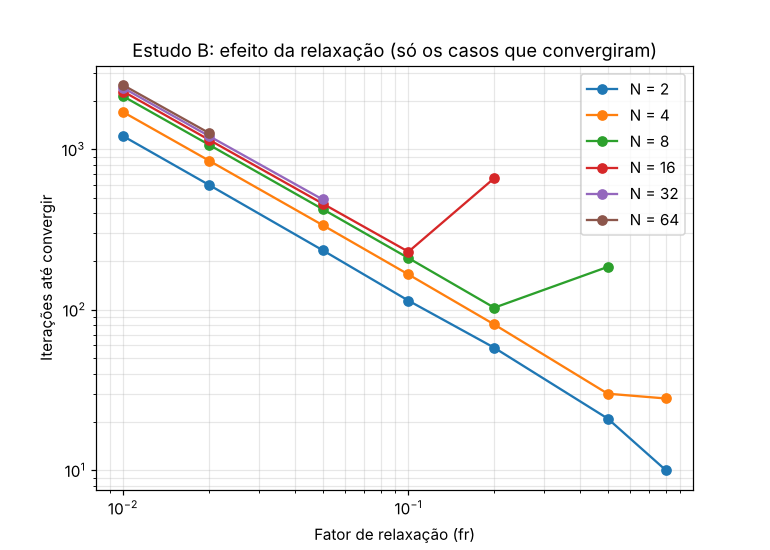
\includegraphics[width=0.55\textwidth]{fig_relaxacao.png}
\caption{Iterações até a convergência em função de $\alpha$. Os pontos
ausentes correspondem a casos que não convergiram.}
\label{fig:relax}
\end{figure}

A Figura~\ref{fig:relax} mostra que o maior $\alpha$ admissível cai de
0,8 ($N=4$) para cerca de 0,02 ($N=64$), aproximadamente com $1/N$. O
SIMPLE despreza $\sum a_{nb}u'_{nb}$, mas aqui $a_W=F_w\approx a_P=F_e$:
o termo desprezado é da ordem do mantido, e a correção de velocidade se
acumula ao longo dos $N$ pontos a montante. O SIMPLE subestima, assim, a
resposta da velocidade à pressão e superestima $p'$, o que exige aplicar
uma fração $\alpha\sim1/N$ da correção. Perto do limite, a solução oscila
antes de convergir (formato em ``V'' das curvas); abaixo dele, as
iterações crescem com $1/\alpha$.

\subsection*{4.2 Estudo de malha}

\begin{table}[H]
\centering
\caption{Estudo de malha sem meio poroso, com o $\alpha$ de menor número
de iterações em cada malha.}
\label{tab:malha}
\begin{tabular}{rrrrrr}
\hline
$N$ & $\alpha$ & Iterações & Tempo (s) & $\dot m$ (kg/s) & Erro (\%)\\
\hline
4   & 0,8   & 28   & 0,0003 & 0,62221 & 39,13\\
8   & 0,3   & 79   & 0,0012 & 0,53032 & 18,58\\
16  & 0,15  & 224  & 0,0046 & 0,48707 & 8,91\\
32  & 0,05  & 487  & 0,0196 & 0,46659 & 4,33\\
64  & 0,03  & 894  & 0,0702 & 0,45674 & 2,13\\
128 & 0,015 & 1824 & 0,2723 & 0,45194 & 1,06\\
256 & 0,007 & 3887 & 1,2122 & 0,44956 & 0,53\\
\hline
\end{tabular}
\end{table}

\begin{figure}[H]
\centering
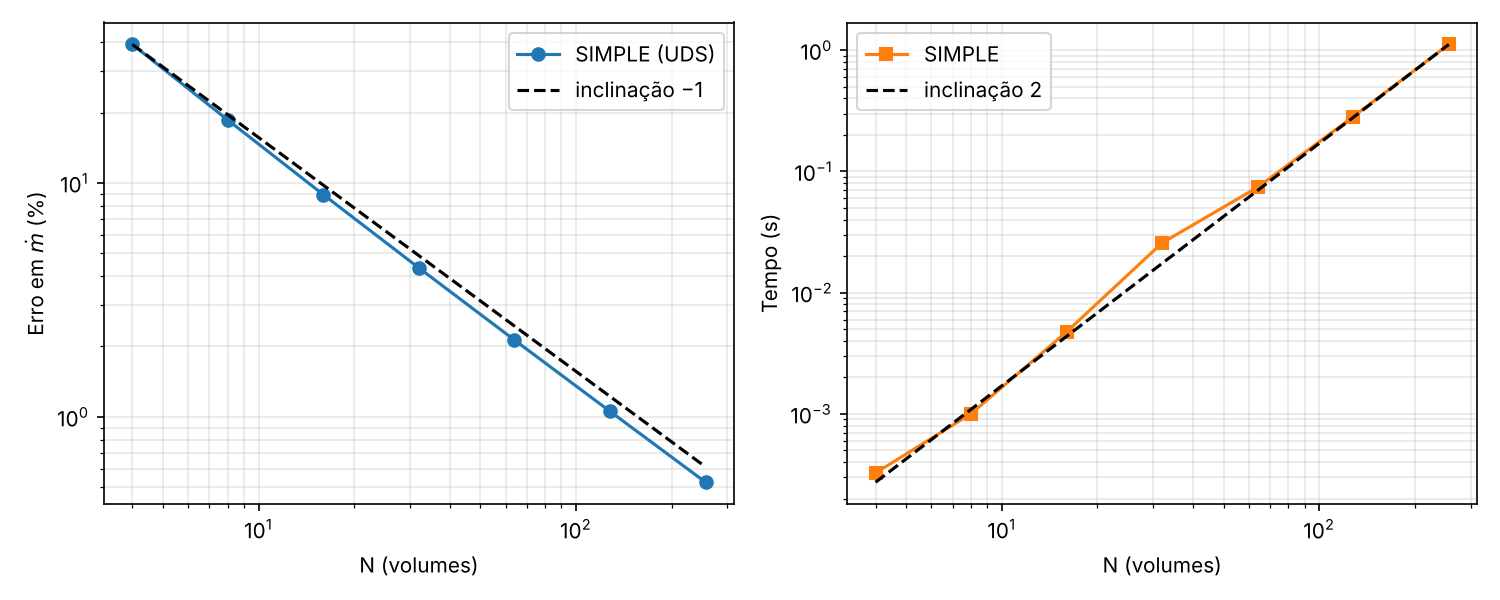
\includegraphics[width=0.8\textwidth]{fig_malha.png}
\caption{Erro na vazão e tempo de processamento em função de $N$.}
\label{fig:malha}
\end{figure}

O erro cai pela metade a cada refino (inclinação $-1$), como esperado para
o UDS, de primeira ordem. As malhas grosseiras superestimam a vazão: o UDS
transporta o momento com a velocidade a montante, inferior à da face em um
escoamento que acelera, subestimando o fluxo de momento na saída. O tempo
cresce com $N^2$, pois o custo por iteração é proporcional a $N$ e o
número de iterações também, devido à redução de $\alpha$: reduzir o erro
pela metade custa quatro vezes mais tempo.

\subsection*{4.3 Critério de convergência}

\pendente{tabela com $\varepsilon_R=10^{-3}$ a $10^{-7}$ para um $N$ fixo:
iterações, tempo e $\dot m$}

\subsection*{4.4 Bocal com meio poroso}

\pendente{validação com a Eq.~\eqref{eq:exata}; estudo de malha e de
sub-relaxação; perfis de $u$ e $p$ com e sem meio poroso}

%======================================================================
\section*{5. Considerações Finais}

\begin{itemize}
  \item O SIMPLE em malha deslocada, com $N$ volumes genérico, reproduziu a
        solução do Exemplo 6.2 de [1].
  \item O erro na vazão é de primeira ordem em $\Delta x$: de 39\% com 4
        volumes a 0,5\% com 256.
  \item O $\alpha$ admissível cai com $1/N$, pois o SIMPLE despreza as
        correções dos vizinhos; com isso, o tempo cresce com $N^2$.
  \item \pendente{critério de convergência e meio poroso}
\end{itemize}

%======================================================================
\section*{6. Referências}

\begin{itemize}
  \item[{[1]}] H.~K. Versteeg e W.~Malalasekera.
        \emph{An Introduction to Computational Fluid Dynamics: The Finite
        Volume Method}. 2.\,ed. Harlow: Pearson, 2007.
  \item[{[2]}] S.~V. Patankar.
        \emph{Numerical Heat Transfer and Fluid Flow}.
        New York: Hemisphere, 1980.
  \item[{[3]}] S.~Ergun.
        Fluid flow through packed columns.
        \emph{Chemical Engineering Progress}, v.~48, p.~89--94, 1952.
  \item[{[4]}] CFD Online. Finite Volume -- SIMPLE Algorithm (fórum).
        Disponível em:\\ \texttt{https://www.cfd-online.com/Forums/main/}\\
        \texttt{16136-finite-volume-simple-algorithm.html}.
\end{itemize}

%======================================================================
\section*{7. Código desenvolvido}

\pendente{substituir pela versão final, com o meio poroso}

{\scriptsize
\begin{verbatim}
# Exemplo 6.2 página 200 livro An Introduction to Computational Fluid Dynamics –
# the finite volume method, 2ª ed. HK Versteeg, W Malalasekera
# Bloco 1: o SIMPLE virou uma função, com limite de iterações,
# checagem de NaN e medição de tempo.

import math
import time
import matplotlib.pyplot as plt

# Dados fixos do problema (não mudam entre as simulações)
rho = 1 # kg/m³
L = 2 # m
A_A = 0.5 # m²
A_E = 0.1 # m²
P_0 = 10 # Pa (pressão de estagnação na entrada)
P_E = 0 # Pa (pressão estática na saída)
m_dot_exato = rho * A_E * math.sqrt(2 * P_0 / rho) # kg/s (Bernoulli)


#TDMA
def tdma(aP, aW, aE, Su):
    n = len(aP)
    P = [0.0] * n
    Q = [0.0] * n

    # Varredura para frente
    P[0] = aE[0] / aP[0]
    Q[0] = Su[0] / aP[0]
    for i in range(1, n):
        den = aP[i] - aW[i] * P[i-1]
        P[i] = aE[i] / den
        Q[i] = (Su[i] + aW[i] * Q[i-1]) / den

    # Substituição pra trás
    u = [0.0] * n
    u[-1] = Q[-1]
    for i in range(n-2, -1, -1):
        u[i] = P[i] * u[i+1] + Q[i]

    return u


def simple(N, fr, err=1e-5, max_it=20000, mostrar=False):
    # N: número de nós de velocidade
    # fr: fator de relaxação
    # err: critério de parada (soma dos resíduos do momento)
    # max_it: número máximo de iterações (proteção contra divergência)
    # mostrar: se True, imprime o resíduo a cada 100 iterações

    dx = L / N # m

    # Malha de pressão
    As_P = [] # Áreas da malha de pressão
    P_cht = [] # Pressões de chute inicial
    for i in range(N + 1):
        As_P.append(0.5 - 0.2 * (i*dx))
        P_cht.append(10 - 5 * (i*dx))

    # Malha de momento
    As_M = [] # Áreas da malha de momento
    m_dot = 1 # kg/s Vazão mássica de chute inicial
    us_cht = [] # Velocidades de chute inicial
    for i in range(N):
        As_M.append(0.5 - 0.2 * (dx/2 + i*dx))
        us_cht.append(m_dot/rho/As_M[i])

    res = 1
    t = [] # histórico dos resíduos
    cont = 0
    convergiu = False

    inicio = time.perf_counter() # marca o tempo de início

    while cont < max_it:
        # Nós internos da malha de velocidades
        Fw = []
        Fe = []
        aW = []
        aE = []
        aP = []
        Su = []
        d = []
        for i in range(1, N-1):
            Fw.append(rho * (us_cht[i] + us_cht[i-1])/2 * As_P[i])
            Fe.append(rho * (us_cht[i] + us_cht[i+1])/2 * As_P[i+1])
            aW.append(Fw[i-1])
            aE.append(0)
            aP.append(aW[i-1] + aE[i-1] + (Fe[i-1] - Fw[i-1]))
            Su.append((P_cht[i] - P_cht[i+1]) * As_M[i])
            d.append(As_M[i]/aP[i-1])
            # (Bloco 3: o arrasto do meio poroso será somado ao aP aqui, antes do d)

        # Condições de contorno
        # Pressão de estagnação (Ponto A)
        uA = us_cht[0] * As_M[0] / As_P[0]
        F_A = rho * uA * As_P[0]
        F_B = rho * (us_cht[0] + us_cht[1]) / 2 * As_P[1]
        aW = [0] + aW
        aE = [0] + aE
        aP = [F_B + F_A / 2 * (As_M[0] / As_P[0])**2] + aP
        Su = [(P_0 - P_cht[1]) * As_M[0] + F_A * (As_M[0] / As_P[0]) * us_cht[0]] + Su
        d = [As_M[0] / aP[0]] + d

        # Pressão ambiente P_E = 0
        F_D = rho * (us_cht[-1] + us_cht[-2]) / 2 * As_P[-2]
        F_E = rho * us_cht[-1] * As_M[-1]
        aW = aW + [F_D]
        aE = aE + [0]
        aP = aP + [aW[-1] + aE[-1] + F_E - F_D]
        Su = Su + [(P_cht[-2] - P_cht[-1]) * As_M[-1]]
        d = d + [As_M[-1] / aP[-1]]

        # Resíduo do momento (com os valores da iteração anterior)
        res = 0
        for i in range(N):
            if i == 0:
                res = res + abs(aP[i] * us_cht[i] - Su[i])
            else:
                res = res + abs(aP[i] * us_cht[i] - aW[i] * us_cht[i-1] - Su[i])
        t.append(res)

        # Checagem de divergência: se o resíduo virou NaN ou infinito, para
        if not math.isfinite(res):
            break

        # Checagem de convergência
        if res < err:
            convergiu = True
            break

        if mostrar and cont != 0 and cont % 100 == 0:
            print(f"Iteração: {cont}   Resíduo: {res}")

        u = tdma(aP, aW, aE, Su)

        # Equações de correção da pressão (nós internos B, C, D...)
        aW_P = []
        aE_P = []
        aP_P = []
        b_l = []
        for i in range(1, N):
            aW_P.append(rho * d[i-1] * As_M[i-1])
            aE_P.append(rho * d[i] * As_M[i])
            aP_P.append(aW_P[i-1] + aE_P[i-1])
            b_l.append(rho * u[i-1] * As_M[i-1] - rho * u[i] * As_M[i])

        P_l = tdma(aP_P, aW_P, aE_P, b_l)

        # Considerando p'_A = p'_E = 0
        P_l = [0] + P_l + [0]

        # Correção de P e de u
        P = [a + b for a, b in zip(P_cht, P_l)]
        for i in range(N):
            u[i] = u[i] + d[i] * (P_l[i] - P_l[i+1])

        # Aplicando o fator de relaxação
        u = [(1-fr) * a + fr * b for a, b in zip(us_cht, u)]
        P = [(1-fr) * a + fr * b for a, b in zip(P_cht, P)]

        # Checagem de divergência: se alguma velocidade explodiu, para
        divergiu = False
        for valor in u:
            if not math.isfinite(valor) or abs(valor) > 1e6:
                divergiu = True
        if divergiu:
            break

        # Pressão em A recalculada por Bernoulli (não é relaxada)
        P[0] = P_0 - rho / 2 * u[0]**2 * (As_M[0]/As_P[0])**2

        us_cht = u
        P_cht = P
        cont += 1

    fim = time.perf_counter() # marca o tempo de fim

    # Vazão mássica (igual em todos os pontos se a continuidade foi satisfeita)
    m_dot = rho * us_cht[-1] * As_M[-1]

    # Junta tudo num dicionário para devolver
    resultado = {
        "N": N,
        "fr": fr,
        "convergiu": convergiu,
        "iteracoes": cont,
        "tempo": fim - inicio,
        "residuos": t,
        "u": us_cht,
        "P": P_cht,
        "m_dot": m_dot,
        "erro_%": (m_dot - m_dot_exato) / m_dot_exato * 100,
        "As_M": As_M,
        "As_P": As_P,
    }
    return resultado


# Teste: problema do livro (N = 4, fr = 0.8)
r = simple(4, 0.8)
print("Convergiu:", r["convergiu"])
print("Iterações:", r["iteracoes"])
print("Tempo (s):", r["tempo"])
print("Vazão (kg/s):", r["m_dot"], "  Exata:", m_dot_exato)
print("Erro (%):", r["erro_%"])
print("u:", r["u"])
print("P:", r["P"])

# Gráfico do resíduo em escala log
plt.semilogy(r["residuos"])
plt.xlabel("Iteração")
plt.ylabel("Soma dos resíduos do momento")
plt.title(f"N = {r['N']}, fr = {r['fr']}")
plt.grid(True)
plt.show()
\end{verbatim}
}